%Talk given at MCQMC 2022 July
\documentclass[11pt,compress,xcolor={usenames,dvipsnames},aspectratio=169]{beamer}
%\documentclass[xcolor={usenames,dvipsnames},aspectratio=169]{beamer} %slides and 
%notes
\usepackage{amsmath,
	amssymb,
	datetime,
	mathtools,
	bbm,
	%mathabx,
	array,
	booktabs,
	xspace,
	multirow,
	calc,
	colortbl,
	siunitx,
 	graphicx}
\usepackage[usenames]{xcolor}
\usepackage[giveninits=false,backend=biber,style=nature,style=authoryear,maxcitenames =10, mincitenames=9]{biblatex}
\addbibresource{FJHown23.bib}
\addbibresource{FJH23.bib}
\usepackage{newpxtext}
\usepackage[euler-digits,euler-hat-accent]{eulervm}
\usepackage{media9}
\usepackage[autolinebreaks]{mcode}
\usepackage[tikz]{mdframed}

\usepackage[T1]{fontenc}
\usepackage{tgadventor} %Font found at https://tug.org/FontCatalogue/
%\usepackage{newpxtext}
\usepackage[euler-digits,euler-hat-accent]{eulervm}


\usetheme{FJHSlimNoFoot169}
\setlength{\parskip}{2ex}
\setlength{\arraycolsep}{0.5ex}

\DeclareMathOperator{\sol}{SOL}
\DeclareMathOperator{\app}{APP}
\DeclareMathOperator{\alg}{ALG}
\DeclareMathOperator{\ACQ}{ACQ}
\DeclareMathOperator{\ERR}{ERR}
\DeclareMathOperator{\COST}{COST}
\DeclareMathOperator{\COMP}{COMP}
\newcommand{\dataN}{\bigl(\hf(\vk_i)\bigr)_{i=1}^n}
\newcommand{\dataNj}{\bigl(\hf(\vk_i)\bigr)_{i=1}^{n_j}}
\newcommand{\dataNjd}{\bigl(\hf(\vk_i)\bigr)_{i=1}^{n_{j^\dagger}}}
\newcommand{\ERRN}{\ERR\bigl(\dataN,n\bigr)}

\newcommand{\Sapp}{S_{\textup{app}}}
\newcommand{\LambdaStd}{\Lambda^{\textup{std}}}
\newcommand{\LambdaSer}{\Lambda^{\textup{ser}}}
\newcommand{\LambdaAll}{\Lambda^{\textup{all}}}
\newcommand{\oton}{1\!:\!n}
\newcommand{\talert}[1]{\alert{\text{#1}}}
\DeclareMathOperator{\init}{init}
\DeclareMathOperator{\GP}{\cg\cp}
\newcommand{\MLE}{\textup{EB}}
\newcommand{\mCtheta}{{\mathsf{C}_{\vtheta}}}
\newcommand{\mCInv}{\mathsf{C}^{-1}}

%\DeclareMathOperator{\app}{app}

\providecommand{\HickernellFJ}{H.\xspace}


\iffalse

Challenges in Developing Great MCQMC Software
Fred J. Hickernell, Illinois Institute of Technology, Chicago, IL USA

The process of translating new Monte Carlo and Quasi-Monte Carlo (MCQMC) algorithms into software libraries faces several challenges.  Great software should be easy to use with reasonable default options for the novice and advanced features for the developer or experienced user.  The library architecture must allow for growth.  Ensuring connectivity with other software libraries will facilitate a larger user base of the MCQMC library.  Coding algorithms the right way may significantly improve their runtime or portability.  Since development team members will come and go, the shared wisdom of the development team must be documented and transmitted to succeeding generations.  Software developers must keep abreast of the newest computing environments to ensure peak performance.  This talk will highlight some of these challenges and ways to address them.


\fi

\renewcommand{\OffTitleLength}{-7ex}
\setlength{\FJHThankYouMessageOffset}{-8ex}
\title{Challenges in Developing Great MCQMC Software}
\author[]{Fred J. Hickernell}
\institute{Department of Applied Mathematics \&
	Center for Interdisciplinary Scientific Computation \\  Illinois Institute of Technology \quad
	\href{mailto:hickernell@iit.edu}{\url{hickernell@iit.edu}} \quad
	\href{http://mypages.iit.edu/~hickernell}{\url{mypages.iit.edu/~hickernell}}}

\thanksnote{with Mark Klinchin and the rest of the GAIL an QMCPy teams \\
	partially supported by SigOpt, an Intel company \\[2ex]
	Thanks to the organizers as we meet again in person in still challenging times\\
	Slides at  \href{https://speakerdeck.com/fjhickernell/quasi-monte-carlo-software}{\nolinkurl{speakerdeck.com/fjhickernell/quasi-monte-carlo-software}}
}
\event{MCQMC 2022}
\date[]{July 18, 2022}

\input FJHDef.tex


\newlength{\figwidth}
\setlength{\figwidth}{0.25\textwidth}

\newlength{\figwidthSmall}
\setlength{\figwidthSmall}{0.2\textwidth}

\newcommand{\financePict}{\href{http://i2.cdn.turner.com/money/dam/assets/130611131918-chicago-board-options-exchange-1024x576.jpg}{\includegraphics[width
		= 3cm]{ProgramsImages/130611131918-chicago-board-options-exchange-1024x576.jpg}}}
	
	\newcommand{\scoop}[1]{\parbox{#1}{
\includegraphics[width=#1]{IceCreamScoop.eps}}\xspace}
	\newcommand{\smallscoop}{\scoop{1cm}}
	\newcommand{\medscoop}{\scoop{1.8cm}}
	\newcommand{\largescoop}{\scoop{3cm}}
	\newcommand{\ICcone}[1]{\parbox{#1}{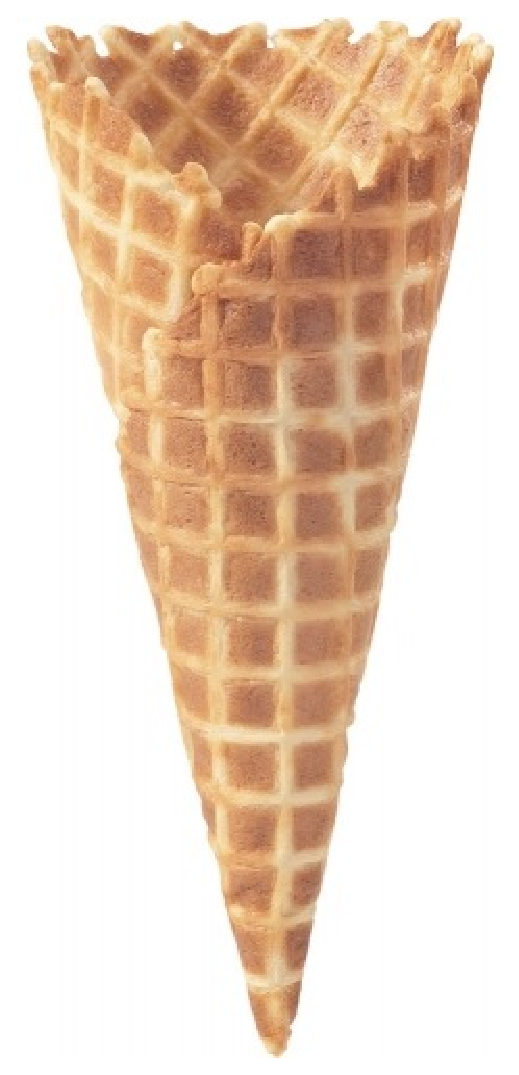
\includegraphics[width=#1,angle=270]{MediumWaffleCone.eps}}\xspace}
	\newcommand{\medcone}{\ICcone{1.2cm}}
	\newcommand{\largercone}{\parbox{2.2cm}{\vspace*{-0.2cm}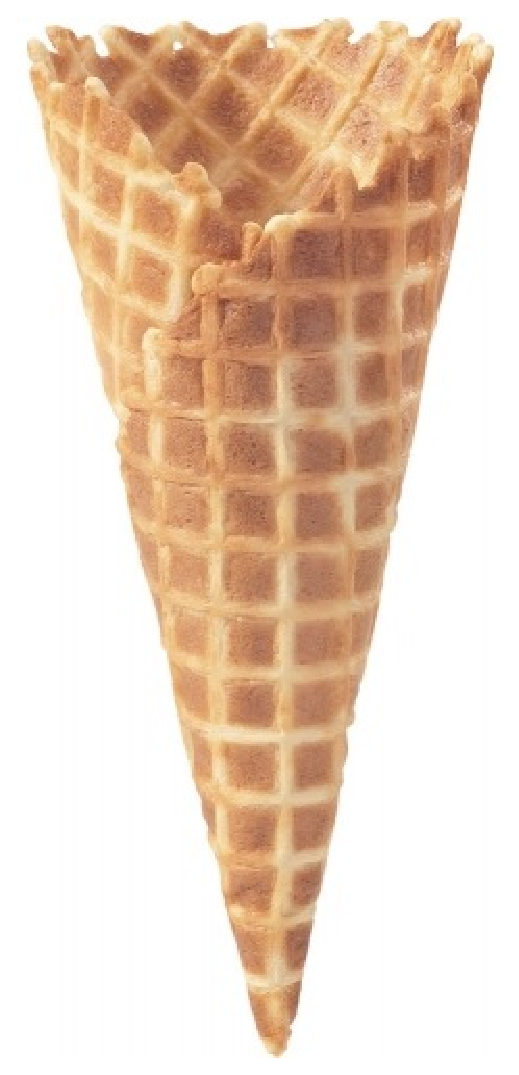
\includegraphics[width=1cm,angle=270]{MediumWaffleCone.eps}}\xspace}
	\newcommand{\largecone}{\ICcone{1.8cm}}
	\newcommand{\smallcone}{\parbox{1.1cm}{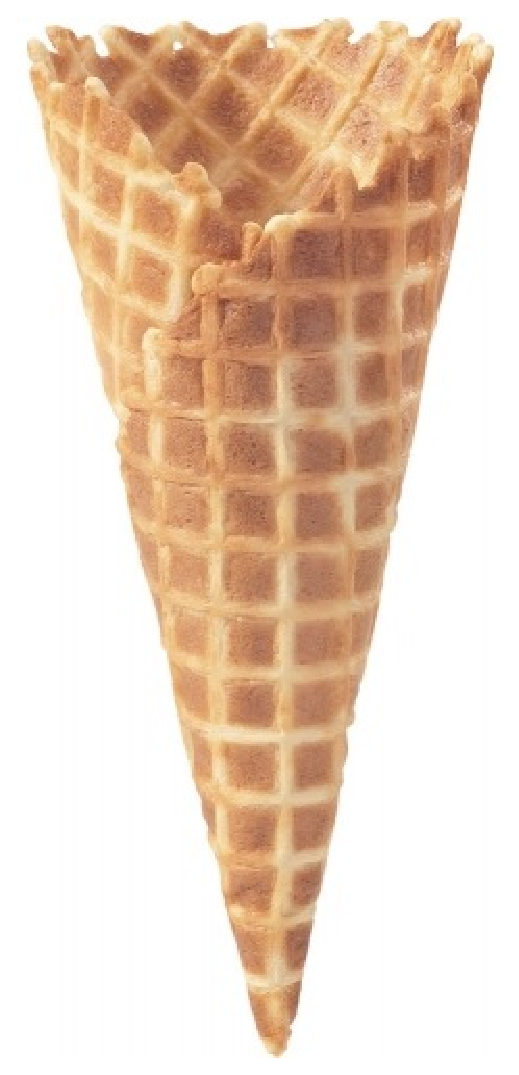
\includegraphics[width=0.5cm,angle=270]{MediumWaffleCone.eps}}\xspace}

	

\newcommand{\northeaststuff}[3]{
	\begin{tikzpicture}[remember picture, overlay]
	\node [shift={(-#1 cm,-#2 cm)}]  at (current page.north east){#3};
	\end{tikzpicture}}


\begin{document}
	\tikzstyle{every picture}+=[remember picture]
	\everymath{\displaystyle}

\frame{\titlepage}


\section{Introduction}

\begin{frame}{My Definition of Great MCQMC Software}
	
	\vspace{-5ex}
	\begin{itemize}
		\item \alert{Correct}, e.g., not omit the zeroth point in a low discrepancy sequence \parencite{Owe22a, scipySobol2020a}
	
		\item  \alert{Complete}---contain the components or have easy access to components in other libraries to solve real, complex problems
		
		\item  \alert{Accessible}---tutorials, demos, discussion forums, etc.\ for (new) users; written in a language that potential users speak; provide a consistent user interface
		
		\item \alert{Efficient}---in terms of compute time and memory
				
		\item \alert{Current}---include the latest and best algorithms

		\item  \alert{Sustainable}--have a sufficient user base and developer community for updates and maintenance
		
		\item \alert{Scalable}--take advantage of latest computer architectures for speed and to tackle large problems
		
	\end{itemize}
\end{frame}

\begin{frame}{Why Do We Need Software?}
\end{frame}

\begin{frame}{Selective History of MC\textbf{QMC} Software}
	\vspace{-4ex}
	\begin{itemize}
		\item \cite{LEc2017a} provides a history of random number generation
		\item Notorious \texttt{randu} \parencite{RANDU}, which failed the spectral test
		\item 
	\end{itemize}
\end{frame}



\printbibliography
\end{document}

\begin{frame}{Quasi-Monte Carlo (QMC) uses low discrepancy (LD) sequences}
	\vspace{-3ex}
	\begin{tabular}{>{\centering}p{0.47\textwidth}@{\quad}>{\centering}p{0.47\textwidth}}
		%Independent \& Identically Distributed (IID) &
		%Low Discrepancy (LD) \tabularnewline
		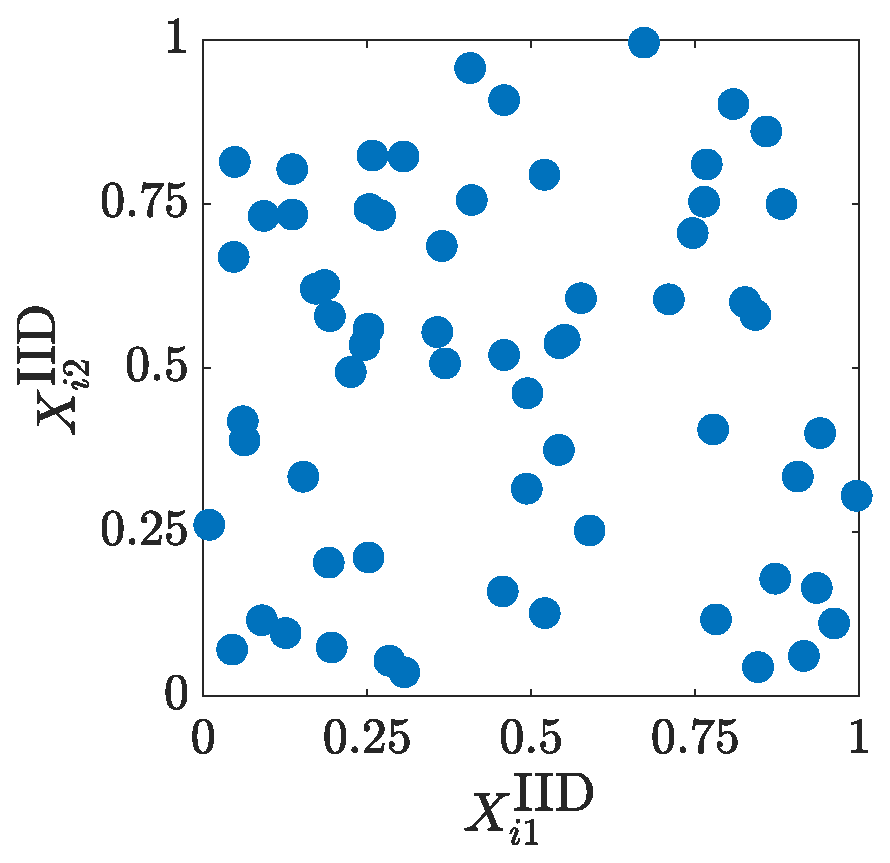
\includegraphics[height=5cm]{ProgramsImages/IIDPoints.eps} &
		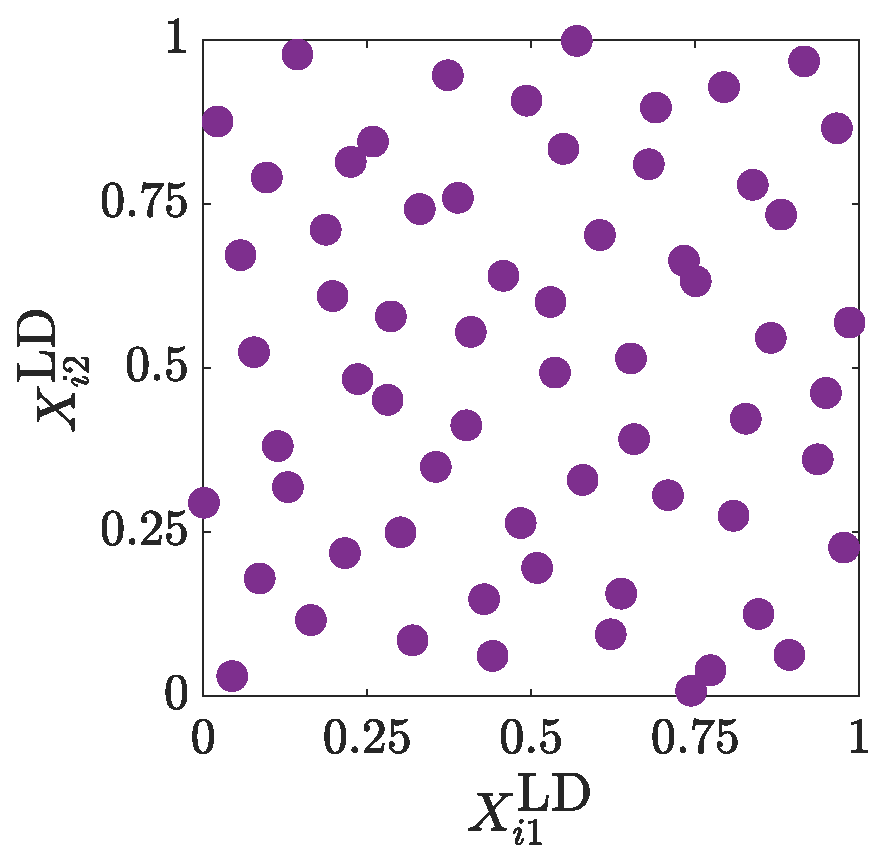
\includegraphics[height=5cm]{ProgramsImages/SSobolPoints.eps}
		\tabularnewline
		$\vT_i$ are random &
		$\vX_i$ may be deterministic \alert{or} random 
		\tabularnewline
		$\vT_1, \vT_2 \cdots \alert{\IIDsim} F$ &
		$\vX_1, \vX_2 \cdots \alert{\LDsim} F$ 
		\tabularnewline
		$\vT_i$ do not know about one another &
		$\{\vX_i\}_{i=1}^n$ represent $F$ well
		\tabularnewline
		$F_{n}(\vt_1, \ldots, \vt_n) = F(\vt_1) \cdots F(\vt_n)$ &
		$F_{\{\vX_i\}_{i=1}^n}(\vx) \approx F(\vx)$
	\end{tabular}
\end{frame}

\begin{frame}{You have heard about QMC.  How do you try it?}
	
	\vspace{-5ex}
\begin{itemize}
\setlength{\itemsep}{0cm}
    \item<1-> \emph{QMC will give you 100 times the accuracy in the same amount of time as simple MC} \\
     \uncover<2->{\alert{Often}}
    \item<1-> \emph{Just replace your IID random points with low discrepancy (LD) points}\\
    \uncover<2->{\alert{Sometimes}}
    
    \vspace{4ex}
    
    \item<3-> \emph{Where can I get accurate, efficient, easy to use QMC software to try for my problem?}\\
     \item<3-> \emph{How can I make my great QMC software available for others?}\\
    \uncover<4->{\alert{Let's try to help}}
    
\end{itemize}
\end{frame}

\begin{frame}{Quasi-Monte Carlo (QMC) uses low discrepancy (LD) sequences}
\vspace{-3ex}
\begin{tabular}{>{\centering}p{0.47\textwidth}@{\quad}>{\centering}p{0.47\textwidth}}
%Independent \& Identically Distributed (IID) &
%Low Discrepancy (LD) \tabularnewline
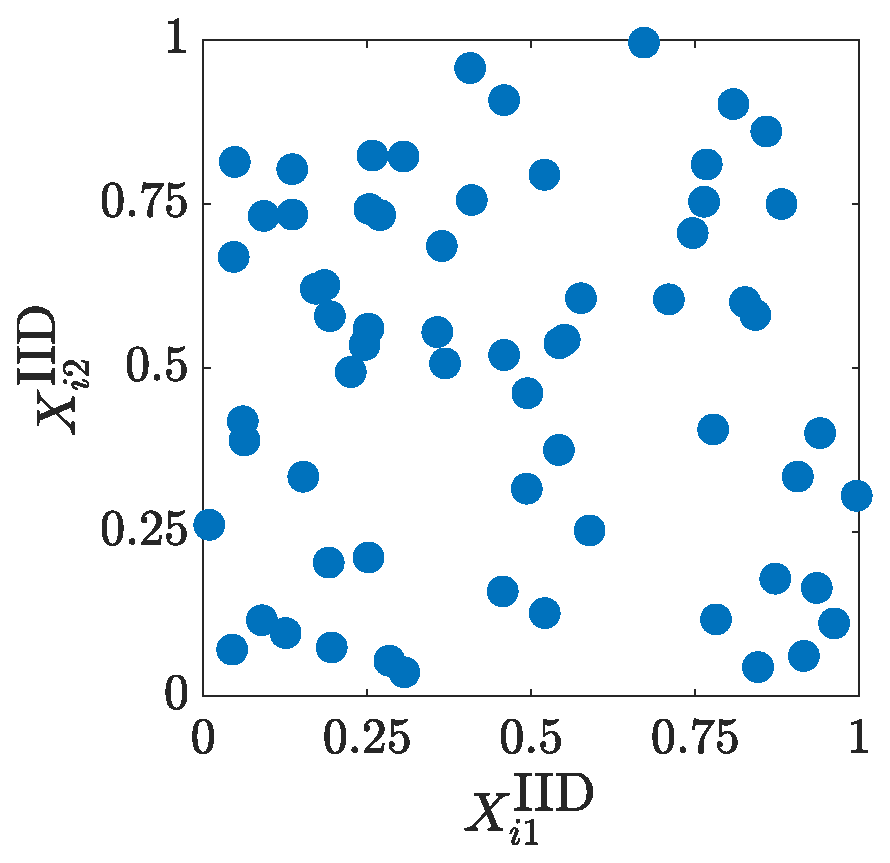
\includegraphics[height=5cm]{ProgramsImages/IIDPoints.eps} &
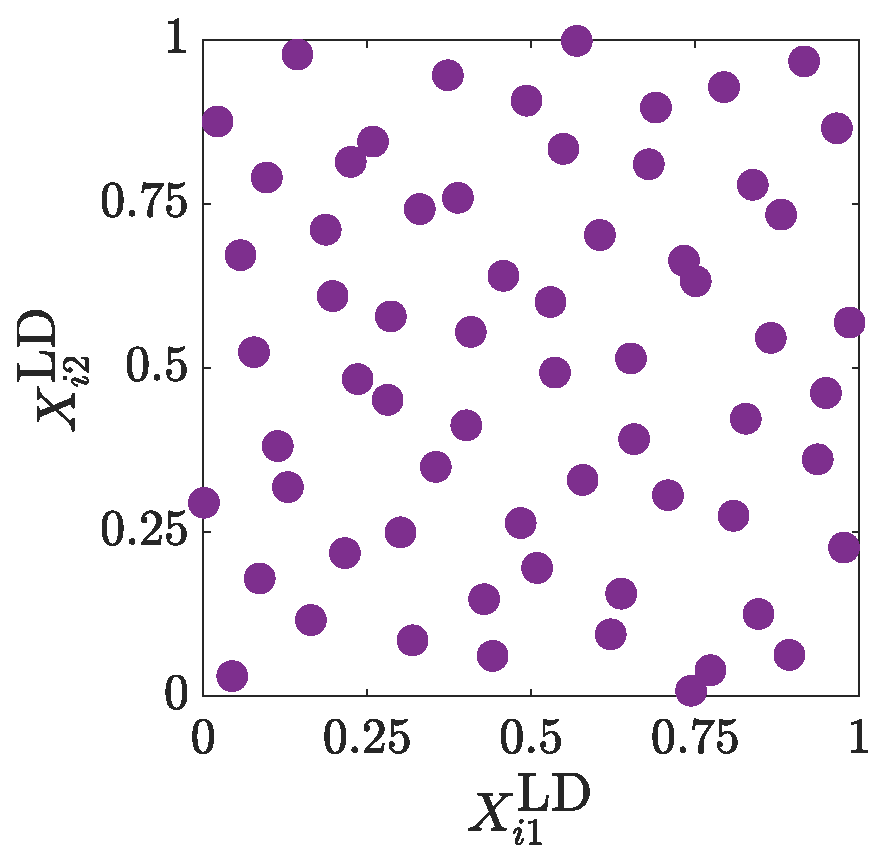
\includegraphics[height=5cm]{ProgramsImages/SSobolPoints.eps}
\tabularnewline
$\vT_i$ are random &
$\vX_i$ may be deterministic \alert{or} random 
\tabularnewline
$\vT_1, \vT_2 \cdots \alert{\IIDsim} F$ &
$\vX_1, \vX_2 \cdots \alert{\LDsim} F$ 
\tabularnewline
$\vT_i$ do not know about one another &
$\{\vX_i\}_{i=1}^n$ represent $F$ well
\tabularnewline
$F_{n}(\vt_1, \ldots, \vt_n) = F(\vt_1) \cdots F(\vt_n)$ &
$F_{\{\vX_i\}_{i=1}^n}(\vx) \approx F(\vx)$
\end{tabular}
\end{frame}

\begin{frame}{Where is the software?  (apologies to those I missed)}
			\vspace{-3ex}
	
	\renewcommand{\arraystretch}{1.15}
	\begin{tabular}{>{\centering}m{0.47\textwidth}@{\qquad}>{\centering}m{0.47\textwidth}}
		\alert{LD Sequence Generators} & \alert{Multi-Level, Stopping Criteria, Applications}
		\tabularnewline \toprule
		\uncover<1>{\href{https://www.mathworks.com}{\alert{MATLAB Statistics Toolbox}}---\newline Sobol' and Halton} &
		\href{https://people.maths.ox.ac.uk/gilesm/mlmc/}{\alert{Mike Giles}}---Multi-Level (Quasi-)Monte Carlo  \uncover<1>{in C++, MATLAB, Python, and R}
		\tabularnewline
		\href{https://cran.r-project.org/web/packages/qrng/qrng.pdf}{\alert{Marius Hofert \& Christiane Lemieux }}---\texttt{qrng} \uncover<1>{R package,} Sobol' and Halton &
	  \href{http://gailgithub.github.io/GAIL_Dev/}{\alert{Guaranteed Automatic Integration Library (GAIL)}}---Stopping criteria  \uncover<1>{in MATLAB}
		\tabularnewline
		\uncover<1>{\href{http://www.broda.co.uk}{\alert{BRODA, Sergei Kucherenko}}---Sobol' in C, MATLAB, and Excel}& 
		\uncover<1>{\href{https://www.uqlab.com}{\alert{UQLab}}---Framework for Uncertainty Quantification in MATLAB}
		\tabularnewline
		\href{http://statweb.stanford.edu/~owen/code/}{\alert{Art Owen}}---randomized Halton\uncover<1>{ in R}&
		\multirow{3}{0.47\textwidth}{\uncover<1>{\centering \href{http://www.openturns.org}{\alert{OpenTURNS}---An Open source initiative for the Treatment of Uncertainties, Risks 'N Statistics in Python}}}
		\tabularnewline
		\uncover<1>{\href{https://github.com/PieterjanRobbe/QMC.jl}{\alert{Pieterjan Robbe}---LD sequences in Julia}}
		\tabularnewline
		\href{https://pytorch.org/}{\alert{PyTorch}---Sobol' \uncover<1>{in Python}}
		\tabularnewline
		\multicolumn{2}{>{\centering}m{0.96\textwidth}}{\href{http://simul.iro.umontreal.ca}{\alert{Pierre L'Ecuyer}---Lattice Builder \uncover<1>{and  Stochastic Simulation in C/C++ and Java}}}
		\tabularnewline
		\multicolumn{2}{>{\centering}m{0.96\textwidth}}{\href{https://people.cs.kuleuven.be/~dirk.nuyens/}{\alert{Dirk Nuyens}}---Magic Point Shop \uncover<1>{and QMC4PDE in MATLAB, Python, and C++}}
\tabularnewline
		\multicolumn{2}{>{\centering}m{0.96\textwidth}}{\uncover<1>{\href{http://people.sc.fsu.edu/~jburkardt/}{\alert{John Burkhardt}}---variety in C++, Fortran, MATLAB, \& Python}}
\tabularnewline
		\multicolumn{2}{>{\centering}m{0.96\textwidth}}{\href{https://qmcsoftware.github.io/QMCSoftware/}{\alert{QMCPy}}---Python package \alert<2->{incorporating and connecting} the work of different groups}
\tabularnewline
	\end{tabular}

\renewcommand{\arraystretch}{1}
    
\end{frame}


\begin{frame}{Why LD is better than IID}
	\vspace{-4ex}
	\begin{description}
		\setlength{\itemsep}{0.5cm}
		\item[Integration/Expectation]  Arising in finance, uncertainty quantification, Bayesian inference, \ldots
		\begin{equation*}
		\mu := \Ex[f(\vX)] = \int_\cx f(\vx) \, \varrho(\vx) \, \dif \vx \approx \frac 1n \sum_{i=1}^n f(\vX_i) =:  \hmu_n
		\end{equation*}
		LD points give faster convergence than IID
		
		\item[Design of Computer Experiments] LD can be more space filling (even than Latin hypercube sampling) for use in constructing surrogate models and uncertainty quantification

		\item[Global Optimization]  LD points are more space filling and find good starting points for local methods
		
		\end{description}
	
    
\end{frame}

\begin{frame}{What software components do we need?}
	
	\vspace{-6ex}
	
	\[
	 \uncover<2->{\mu :=  \int_{\ct} \alert<3>{g(\vt)} \, \alert<2>{\lambda(\vt) \, \dif \vt} = \cdots = } \only<1>{\mu :=} 	\underbrace{\Ex[f(\vX)]}_{\text{expectation}} = \underbrace{\int_\cx \alert<3>{f(\vx)} \, \varrho(\vx) \, \dif \vx}_{\text{integration}} \approx  \frac 1{\alert<4>{n}} \sum_{i=1}^{\alert<4>{n}} f(\alert<1>{\vX_i}) =: \hmu_{\alert<4>{n}}
	\]
	
		\vspace{-3ex}
	
	\begin{description}[<+->]
				\setlength{\itemsep}{0.5cm}
		
		\item[LD Generator] producing $\{\vX_1, \vX_2, \dots \}$ that mimics the distribution with PDF $\varrho$, e.g., uniform
		
		\item[True Measure] that defines the original integral, e.g., Lebesgue
		
		\item[Integrand] $g$, which defines the original integral, plus the transformed version, $f$, to fit the LD generator
		
		\item[Stopping Criterion] that determines how large $n$ should be to ensure that $\abs{\mu - \hmu_n} \le \varepsilon$
	\end{description}
\end{frame}

\section{QMCPy on Google Colaboratory}
\begin{frame}{QMCPy in a Jupyter Notebooks on Google Colaboratory}
	\vspace{-4ex}
	
	\alert{Prerequisites}---No Python, Jupyter, or QMC knowledge assumed
	
	\vspace{-1ex}
	
	\alert{Goals}
	
		\vspace{-3ex}
		\begin{itemize}
		\item Show you how QMC software works
		\item Interest you in using/contributing
	\end{itemize}
	
	\vspace{-1ex}

	\alert{Directions}
	
	\vspace{-3ex}
	\begin{itemize}
		\item Point your browser to \href{https://tinyurl.com/QMCPyTutorial}{\nolinkurl{https://tinyurl.com/QMCPyTutorial}}
		\item Open the file in Google Colaboratory (may need to push a button at the top of your browser)
		\item Make a copy of this file onto your own Google drive account \\
		\texttt{File} $\rightarrow$ \texttt{Save a copy in Drive}
	\end{itemize}



\alert{Pause for questions}
\end{frame}

\section{Why collaborate?}

\begin{frame}
	\frametitle{Acknowledgments for QMCPy}
	
	\begin{itemize}
		\item Coded almost entirely by Aleksei Sorokin (BS/MS '21)
		
		\item Relies on code from several groups (see above)
		
		\item Documentation and testing by Sou-Cheng Choi and Jagadeeswaran R.
		
		\item Funded and encouraged by Mike McCourt at SigOpt
	\end{itemize}
\end{frame}


\begin{frame}
	{The Guaranteed Automatic Integration Library (GAIL) and QMCPy teams}
	
	\vspace{-2ex}
	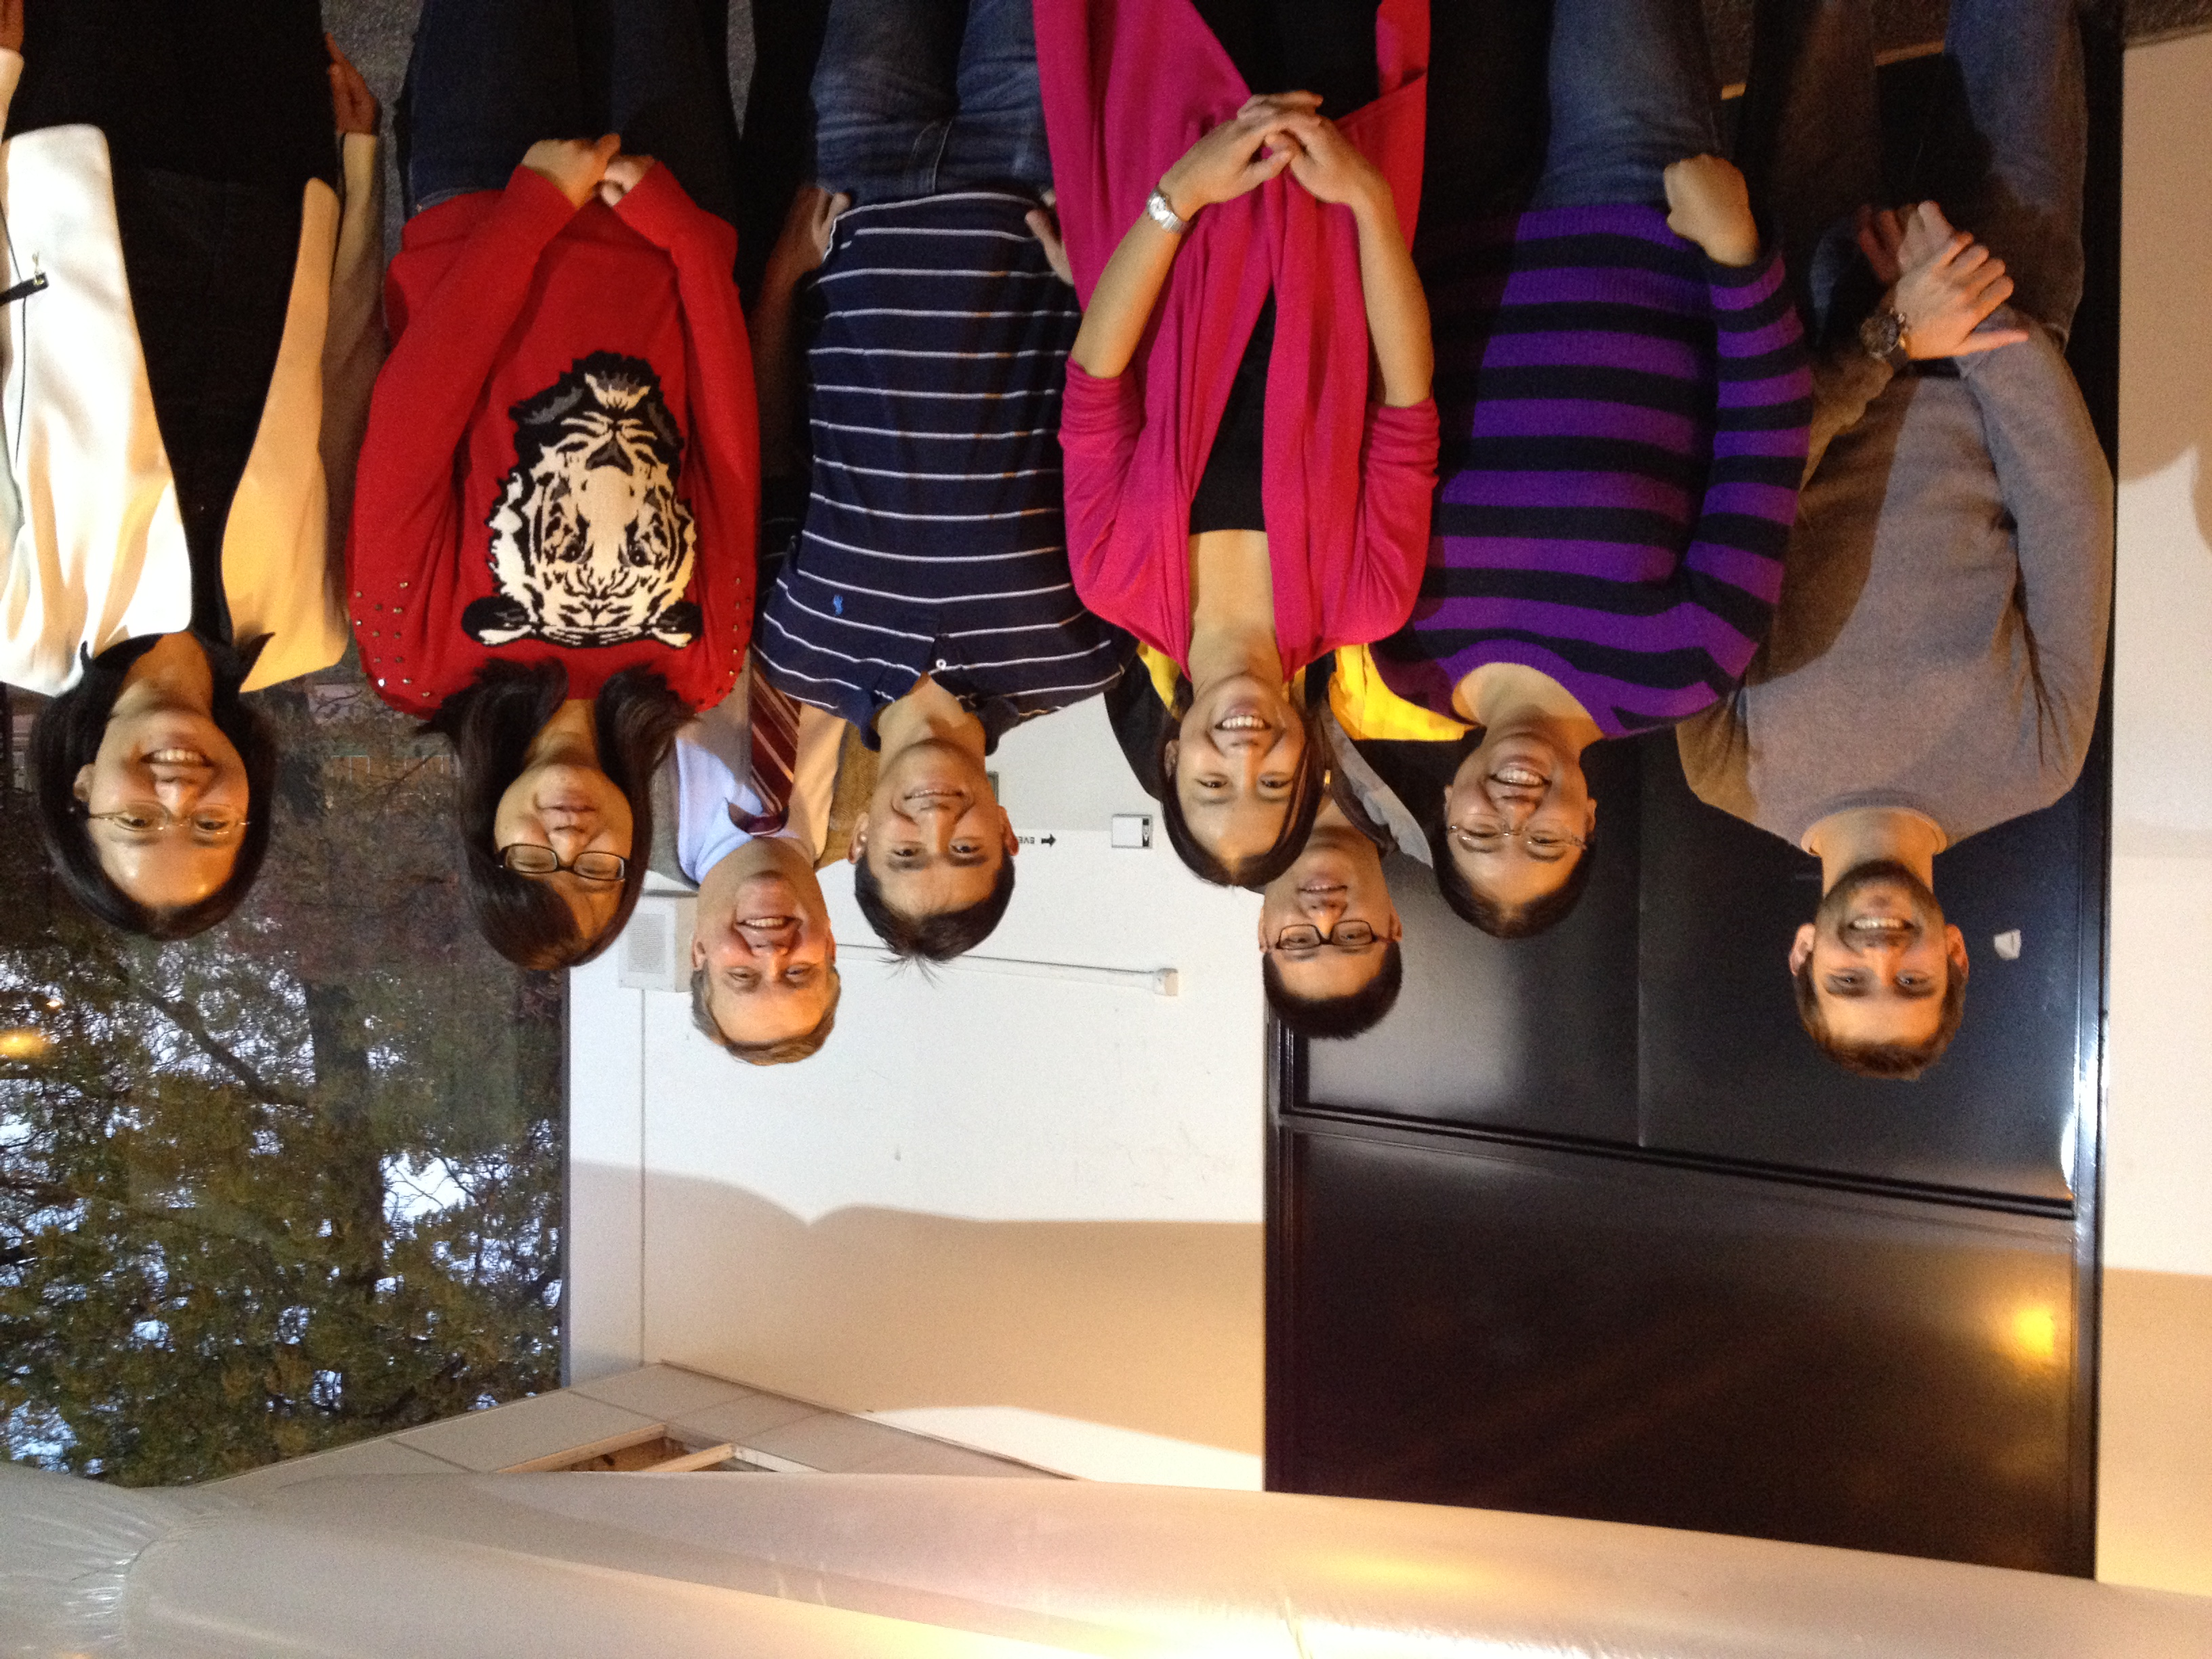
\includegraphics[angle = 180, origin = c, width = 0.32\textwidth]{ProgramsImages/GAIL2014RE.jpeg} \
	
\includegraphics[width = 0.32\textwidth]{ProgramsImages/GAILatSIAM2018Hi.jpeg} \ 
	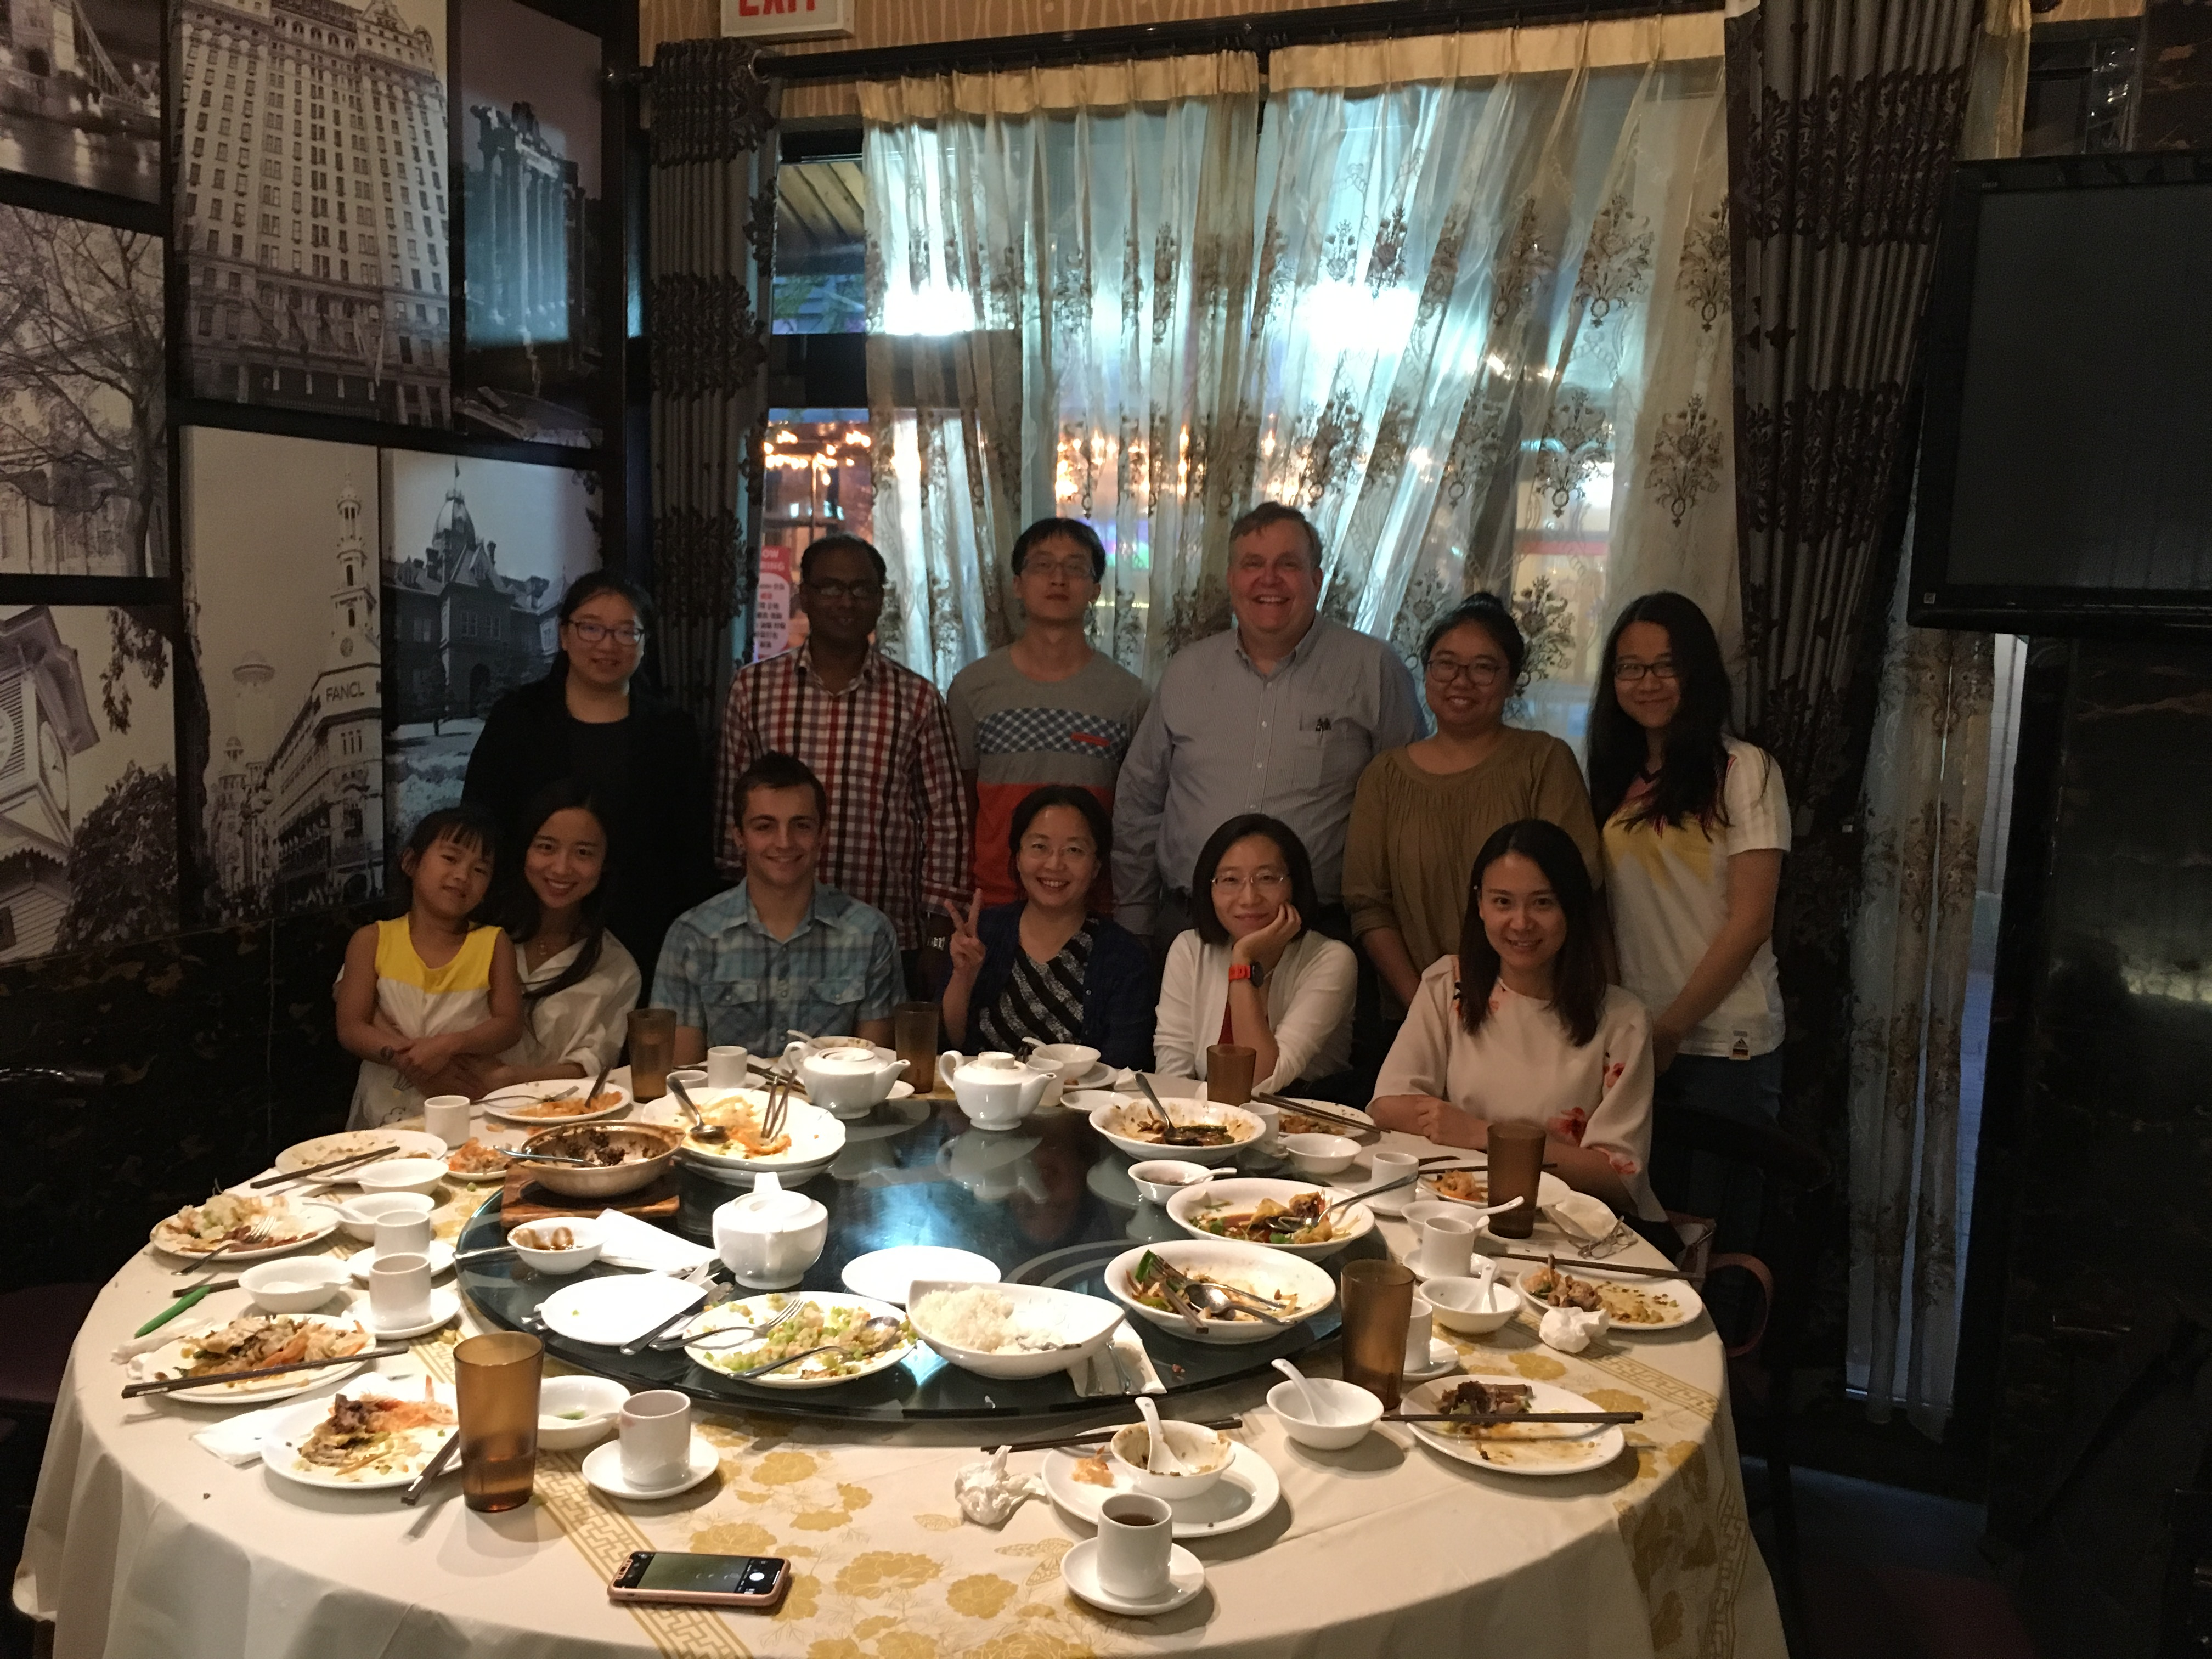
\includegraphics[width = 0.32\textwidth]{ProgramsImages/GAILatChinatown2018.jpg}
	
	\vspace{-4ex}

	{\small 
		\hspace{-4ex}\begin{tabular}{p{0.545\textwidth}p{0.44\textwidth}}
		
		\begin{itemize}
			\setlength{\itemsep}{0ex}
	
			\item Sou-Cheng Choi (Chief Data Scientist, Kamakura)
			
			\item Yuhan Ding (IIT PhD '15, Lecturer, IIT)
			
			\item Lan Jiang  (IIT PhD '16, Compass)
			
			\item Llu\'is Antoni Jim\'enez Rugama (IIT PhD '17, UBS)
			
			\item Mike McCourt (IIT BS '07, Cornell PhD '12, \\ Head of Research, SigOpt)
			
			\item Jagadeeswaran Rathinavel (IIT PhD '19, Wi-Tronix)
			
			
			
			
		\end{itemize}
		
		&
		
		\begin{itemize}
			
			\setlength{\itemsep}{0ex}
			
			\item Aleksei Sorokin (IIT BS \& MAS '21 exp.)
			
			\item  Xin Tong (IIT MS, UIC PhD '20 exp.)
			
			\item Kan Zhang (IIT PhD '20 exp.)
			
			\item Yizhi Zhang (IIT PhD '18, Jamran Int'l)
			
			\item Xuan Zhou (IIT PhD '15, JP Morgan)
			
			\item and others
			
			
		\end{itemize}
	
		
	\end{tabular}
}

\end{frame}

\begin{frame}{The argument for community software}
	
	\vspace{-4ex}
	
	\begin{itemize}
	\item<+-> Our research groups are typically expert at only part of the whole picture:
			\begin{itemize}
			\item LD sequence generators
			
			\item Increasing efficiency, e.g., MLMC, MDM
			
			\item Stopping criteria
			
			\item Use cases
		\end{itemize}
	
		A community library lets us all take advantage of the best

	\item<+-> Provides a consistent interface for pieces from different places
	
	\item<+-> Enables reproducible computational research
	
	\item<+-> Tedious stuff only done once

		\item<+-> Many eyes find and correct errors
		\begin{itemize}
			\item MATLAB's Sobol' generator's  scrambling corrected in MATLAB 2017a after Tony Jim\'enez Rugama noticed the problem
			
			\item PyTorch's Sobol' generator found to be wrong unless double precision is proactively specified; also missing the first point; reported at \url{https://github.com/pytorch/pytorch/issues/32047}
		\end{itemize}
	

\end{itemize}
\end{frame}

\begin{frame}{How you can contribute}
	
		\vspace{-3ex}
	Try out  QMCPy and then
	
			\vspace{-1ex}
	
	
	\begin{description}
		\item[Easy] Submit your bugs and feature requests as issues to \url{https://github.com/QMCSoftware/QMCSoftware/issues}
		
		\item[Moderately Difficult]  Ask your students or collaborators to try QMCPy themselves and submit their bugs and feature requests\\[1ex]
		
		Email us your blog post to add to \href{https://qmcpy.wordpress.com/}{\nolinkurl{qmcpy.wordpress.com/}}
		
		\item[Heroic] Add a feature or use case and make a pull request at \url{https://github.com/QMCSoftware/QMCSoftware/pulls} \\ so that we can included it in our next release
	\end{description}

		\vspace{-1ex}
	
	Questions or suggestions?  Email us at \href{mailto:qmc-software@googlegroups.com}{\nolinkurl{qmc-software@googlegroups.com}}
	
			\vspace{-1ex}
	
	\uncover<2>{If you are wedded to another language, think of designing your software so that others can add to it easily.}

\end{frame}

\finalthanksnote{These slides are  available at \\  \href{https://speakerdeck.com/fjhickernell/quasi-monte-carlo-software}{\nolinkurl{speakerdeck.com/fjhickernell/quasi-monte-carlo-software}}\\
Google Colaboratory notebook at \href{https://tinyurl.com/QMCPyTutorial}{\nolinkurl{tinyurl.com/QMCPyTutorial}}\\
Blog at \href{https://qmcpy.wordpress.com/}{\nolinkurl{qmcpy.wordpress.com/}}}


\thankyouframe


\end{document}





